\chapter{Implementation}

This chapter details the implementation of Snapstore. This includes data structures and the synchronization algorithm. 

Snapstore was built to be cross-platform using Electron\footnote{http://electron.atom.io/}. We used web sockets\footnote{www.socket.io} for networking. Once a client is connected over a socket, Snapstore can constantly pull in and push out new events that come in from that user and from other users. Sockets provide the additional benefit of allowing us to group users. We used this functionality to make ``rooms'' of users that have read and write access to a specific branch, allowing us to push out changes on that branch.

\section{Data Structures}

\subsection{Client}

Each local repository on the client has its own Mongo\footnote{https://www.mongodb.com/} database. Each database has a collection of snapshots, branches, groups, tags, and events. It also has one snapstore document and a binary large object (blob) collection. A data model, using a simplfied entity relationship notation, representing each data structure and its attributes is shown in figure 4-1. 

In this diagram (and in the diagram for the server's data structures), attributes in a data structure are connected to another attribute of a data structure if they are references to that attribute. Each relationship is either a one-to-one relationship -- notated by a a straight line -- or a one-to-many relationship -- notated by a line with an end that splits into three lines. For example, a snapshot can have multiple parents, so there is a one-to-many relationship between the ``parent'' attribute and the ``id'' attribute. On the other hand, a snapshot can only have one child, so there is a one-to-one relationship between the ``child'' attribute and the ``id'' attribute.

\begin{figure}
\includegraphics[max width= \linewidth]{DataModel}
\caption{Snapstore client data model.}
\label{arm:fig1}
\end{figure}

When a file is saved, the resulting snapshot must first decide what kind of snapshot it is. Whether it is a create, update, rename, delete, merge, or conflict snapshot dictates how it will populate its data fields. A create snapshot, for example, has no parent snapshot. When a snapshot is created, it is added to the snapshot collection, and its branch updates its head snapshots to include the new snapshot, while removing its parent. To read the history of a file, the head snapshot of the file is located, and the rest is found by searching backwards through the snapshot graph.

If two snapshots have the same content, they point to the same blob data in the blob collection to save space. This blob collection holds hashes of the content along with the binary content.

When a new branch is created, it is added to the database with only a name. If, however, it was cloned from another branch, the cloned branch will point to all head snapshots, groups, and tags from the original branch. When switching to a branch, the heads snapshots for the target branch are read and applied to the Snapstore folder.

The event collection stores all of the snapshots, groups, and tag events on the client that have not been confirmed by the server. As these events are confirmed, they are erased from the collection.

\subsection{Upstream}

On the upstream server, the snapshot, branch, group, tag, and content data structures are the exact same as those on the client. They are kept consistent with each local repository when a socket connection is open. A model of the data structures on the upstream is shown in figure 4-2.

\begin{figure}
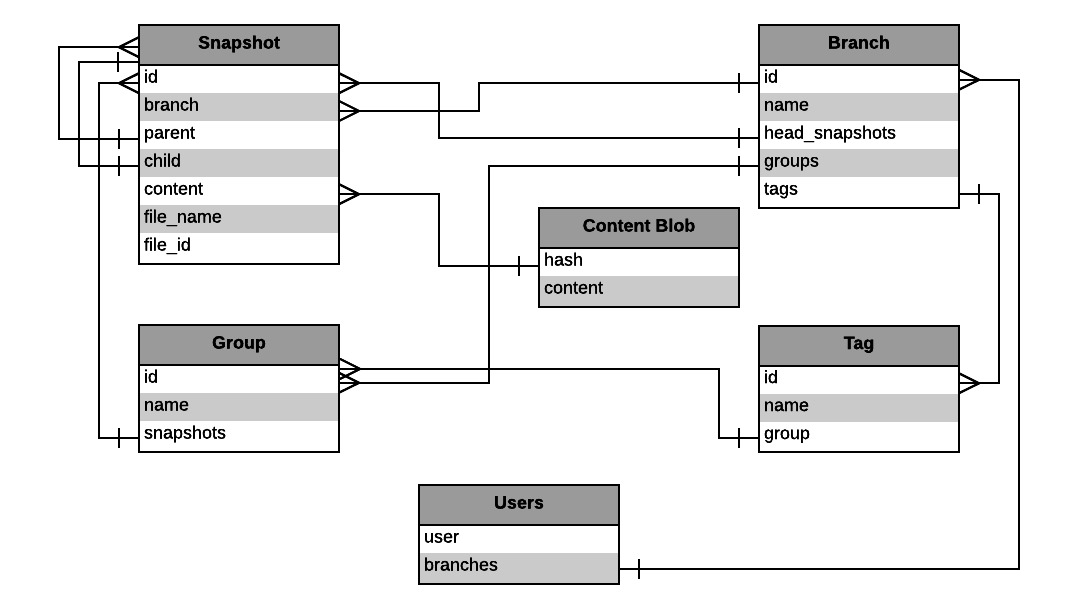
\includegraphics[max width= \linewidth]{DataModelServer}
\caption{Snapstore server data model.}
\label{arm:fig1}
\end{figure}

The user model on the server is a mapping of users to branches to which they have access. When a user shares a branch with another user, that branch is added to this mapping for that user. The server uses this mapping to share data with the appropriate users.

\section{Keeping Data in Sync}

In Snapstore, users can work on a shared branch. As described in section 2.2.3, a shared branch is a line of development where a change from one user is propagated to all other users who are collaborators on that branch, keeping all of their Snapstore folders consistent.

However, this workflow can be difficult to maintain. Multiple users can be making edits at the same time, increasing concurrency issues. If two snapshots are made at the same time, for example, the snapshot graph must be resolved and distributed to all clients. Also, a user can go offline and create snapshots, while their shared files are being written to by other, online users. Snapstore should be able to handle their reintroduction to the network without destroying the snapshot graph.

It is also important to maintain the ordering of events created by a single user. If a user creates a snapshot and then creates a group with that snapshot it in, it is necessary to send those two events in order to the server. Otherwise, the server might, for example, try to create a group containing a snapshot that doesn't exist.

We take the approach that any event that reaches the upstream server and is confirmed should be regarded as correct for the entire system. This means that it should never be undone or modified, even if a conflicting event arrives. This also means that all clients can safely save every event that comes from the server. Using this idea, we designed a protocol algorithm for this process, called Distributed Event Synchronization Queue (DESQ).

Each client has their own ordering of events, or database operations, that are stored in a client queue until they are confirmed by the server. DESQ seeks to reach eventual consistency between these queues so that every client on a shared branch has the same data.


\begin{center}
\begin{figure}[ht]
\begin{algorithmic}[1]
\State $events \gets \text{pointer to }Events \text{ collection}$
\State $socket \gets \text{server socket connection}$
\Function{Database-Listener}{}
\While {new database action \emph{event} by user}
\State $events\text{.append(}event\text{)}$
\EndWhile
\EndFunction
\Function{Events-Listener}{}
\While {new \emph{event} added to \emph{Events} collection}
\State $\text{Client-DESQ()}$
\EndWhile
\EndFunction
\Function{Network-Listener}{}
\While {network connection with server established}
\State $socket\text{.send("Check For New Events")}$
\State $\text{Client-DESQ()}$
\EndWhile
\EndFunction
\Function{DESQ-Response}{}
\While { \emph{socket}.response(\emph{response, event, message})}:
\If {$message == \text{"Confirmed" or "Duplicate"}$}
\State $events\text{.remove(}event\text{)}$
\ElsIf {$message == \text{"Reject"}$}
\If {$event\text{.type} == \text{Snapshot}$} \Comment{response is a list of snapshots}
\State Save \emph{response} \Comment{these snapshot events fix the conflict}
\State $event\text{.data.parent} = response\text{.head}$
\EndIf
\Else \Comment{$message == \text{"New Event"}$}
\If {$response.data.parent \text{ is not a head snapshot}$}
\State \textbf{return}
\EndIf
\State Save \emph{response}
\EndIf
\EndWhile
\EndFunction
\Procedure{Client-DESQ}{}
\For {$\text{each } event\text{ in } events \text{ collection}$}
\If {network connection is lost}
\State \textbf{break}
\EndIf
\State $socket\text{.send(}event\text{)}$
\EndFor
\EndProcedure
\end{algorithmic}
\caption{Client-DESQ pseudocode}\label{euclid}
\end{figure}
\end{center}

\subsubsection{Client}

Client-DESQ, whose pseudocode is in Figure 4-3, can be triggered in one of two ways. Either a database action has occurred (listener defined on line 3), or a network connection with the server has been established (listener defined on line 9). 

Once Client-DESQ is called, it cannot be called again until it has finished sending each event in the list. This is because Snapstore was implemented in javascript, which uses an single-threaded event loop. While Client-DESQ is running, events can be \textit{queued up} to be added to the event list, but they won't actually be added. This effectively locks the event list. It is important to not add any new events to the event list while Client-DESQ is running because these events could be missed and not sent until another added event triggers Event-Listener.

If Client-DESQ is started via network connection, the client first queries the server to see if there are any new events the client needs (line 11). If there are, the server sends them back as a ``New Event'', and the client saves them (line 24).

Once Client-DESQ begins, it sends each event in the event list to the server in order (line 29). Because this communication is happening on a socket over TCP, these events are guaranteed to arrive in order, the same order they were created in the client.

If an event is confirmed by the server, or if it is a duplicate event, the client removes this event from their event collection (lines 15-16). 

If an event is rejected by the server, the client responds in one of two ways. If the rejected event is a snapshot event, the client saves the snapshots that will fix the conflict and updates the event snapshot's parent to be the head (lines 18-20). If the rejected event is a group or a tag event, nothing needs to be done; the event stays in its current location in the event collection.

During Client-DESQ, if the network connection is lost, the process stops (lines 27 and 28). No events are discarded or lost when this happens, but the process terminates so that it can begin fresh once a connection is restored. The event is left in its same location in the list, maintaining the event list's order.

A non-obvious statement appears on line 22, and it handles the following situation. A client, Alice, sends a snapshot to the server at the same time as Bob. Alice's snapshot is confirmed and sent to Bob. Bob's snapshot is then rejected. Alice's snapshot will then be sent to Bob twice, once by the ``New Event'' response, and once by the ``Reject'' response. To mitigate this, we ignore any snapshot ``New Event'' response whose parent is not a head on the client. In this case, that head is Bob's rejected snapshot. The client discards any events from the server that cause a conflict on the client because the client knows that a resolution to that conflict must be on its way.

This scenario can be understood by looking at Figure 2-5 in section 2.2.3. Once Alice's snapshot 3 is confirmed by the sever, it will be sent to Bob as a ``New Event''. However, Bob will discard this snapshot because it's parent, 1, is not the head snapshot on Bob's client, 2. The eliminates Bob saving snapshot 3 twice; he only saves it once the ``Reject'' response arrives.

\begin{center}
\begin{figure}[h]
\begin{algorithmic}[1]
\Procedure{Server-DESQ}{}
\State $\textit{socket} \gets \text{client socket connection}$
\State $\textit{eventMap} \gets \text{persistent storage of unsent events}$
\While {\emph{socket}.receive(\emph{event})}:
\If {$event \text{ == "Check For New Events"}$}
\State $newEvents \gets eventMap[socket.user]$
\If {$newEvents\text{.size() } != 0$}
\State $socket\text{.send(}newEvents, \text{"New Event")}$
\State $eventMap[socket.user] = []$
\EndIf
\ElsIf {$\textit{event} \text{.data.id in database}$}
\State $socket\text{.send(}event, \text{"Duplicate")}$
\ElsIf {$\textit{event}\text{.type } == \text{Group}$}
\If {$event\text{.data.snapshots in database}$}
\State $\text{Confirm-Event(}event, socket, eventMap\text{)}$
\Else 
\State $socket\text{.send((), event, "Reject")}$
\EndIf
\ElsIf {$\textit{event}\text{.type } == \text{Tag}$}
\If {$event\text{.data.group in database}$}
\State $\text{Confirm-Event(}event, socket, eventMap\text{)}$
\Else 
\State $socket\text{.send((), event, "Reject")}$ 
\EndIf
\Else \Comment{$event\text{.type } == \text{Snapshot}$}
\If {$event\text{.data.parent is head snapshot}$}
\State $\text{Confirm-Event(}event, socket, eventMap\text{)}$
\Else
\State $conflictSnapshots \gets \text{All snapshots between }event\text{.parent and }head$
\State $socket\text{.send(}conflictSnapshots, event\text{,"Reject")}$
\EndIf
\EndIf
\EndWhile
\EndProcedure
\Procedure{Confirm-Event}{event, socket, eventMap}
\State $socket\text{.send(}event, \text{"Confirm")}$
\State $\text{save }event\text{ in database}$
\For {each \emph{user} with access to \emph{event}.branch}
\If {\emph{user} is connected}
\State $socket\text{(}user\text{).send(}event, \text{"New Event")}$
\Else
\State \emph{eventMap}[\emph{user}].append(\emph{event})
\EndIf
\EndFor
\EndProcedure
\end{algorithmic}
\caption{Server-DESQ pseudocode}\label{euclid}
\end{figure}
\end{center}

\subsubsection{Server}

Server-DESQ, whose pseudocode is in Figure 4-4, begins on the server when it receives an event over the socket from a client. If this event is the message ``Check For New Events'', the server looks in its storage of unsent events for that user and sends them (lines 5-9). If the event is not ``Check For New Events'', it must be an snapshot, group, or tag event.

If the server has already seen the event, it is flagged as a duplicate (line 11) and returned to the client. 

An event is confirmed if it can be applied to the server's database without triggered any causality issues (discussed in the following paragraph) in the data. When an event is confirmed, it is first returned to the client who sent it. After that, the event must be propagated to all collaborators of the event's creator. The server finds all users that have access to that event's branch (line 31). For each of those users, they are either online and can be forwarded the event (line 32-33), or they are offline and the event must be stored for them (line 34-35). Any collaborator that receives this event can apply it to their local repository because it is a confirmed event coming from the server.

%Reject
Events are rejected if they cause a conflict in causality on the server. The logic which detects this causality conflict for the group event, the tag event, and the snapshot event (lines 13, 18, and 23, respectively) make up a strict ordering of events for Snapstore. This allows Snapstore to use the ``happened before'' relationship between system events \cite{Lamport}. Any event that requires that another, unseen or incorrectly ordered, event ``happened before'' is rejected. If this rejected event is a group or a tag, only a rejection message is sent because the client will eventually send the snapshots or group that will fix the conflict (lines 16 and 21). If the rejected event is a snapshot, other snapshots that will fix the inconsistencies are returned to the client (lines 26-27). 

In Git terms, if there is a conflict in a snapshot graph, the graph rebases and Snapstore tries to push that snapshot again. The rebasing keeps the snapshot graph and the workflow for the branch linear. However, while Git creates new commits during a rebase, Snapstore uses existing snapshots.


